\documentclass[conference]{IEEEtran}
\IEEEoverridecommandlockouts

% IEEEtran requests Times (ptm). Under a Unicode engine (XeTeX/tectonic) there are
% no ptm shapes, so the paper silently falls back to Latin Modern; TeX Gyre Termes
% is a metric-compatible Times clone that restores the required IEEE face. Under
% pdfLaTeX (e.g. Overleaf, IEEE PDF eXpress) ptm resolves natively and this branch
% is skipped.
\usepackage{iftex}
\ifPDFTeX
  \usepackage[T1]{fontenc}
\else
  \usepackage{fontspec}
  \setmainfont{texgyretermes}[
    Extension=.otf,
    UprightFont=*-regular,
    BoldFont=*-bold,
    ItalicFont=*-italic,
    BoldItalicFont=*-bolditalic]
\fi

\usepackage{cite}
\usepackage{amsmath,amssymb,amsfonts}
\usepackage{graphicx}
\usepackage{booktabs}
\usepackage{textcomp}
\usepackage{xcolor}
\usepackage{balance}
\usepackage{tikz}
\usetikzlibrary{positioning,arrows.meta,fit,backgrounds}
\usepackage{pgfplots}
\pgfplotsset{compat=1.17}
\usepackage[hidelinks]{hyperref}

\newcommand{\udm}{PhyUDM}
\newcommand{\condA}{A}
\newcommand{\condB}{B}
\newcommand{\condC}{C}
\newcommand{\condG}{G}
\newcommand{\hs}{\texttt{health\_scan}}
\newcommand{\todo}[1]{\textcolor{red}{[TODO: #1]}}

\begin{document}

\title{Does a Vendor-Neutral Data Model Help LLMs Diagnose Robot Faults?
A Paired Benchmark of Unified Telemetry over the Model Context Protocol}

\author{\IEEEauthorblockN{Christopher A. Herczeg}
\IEEEauthorblockA{\textit{Founder, PhyWare Labs} \\
Chicago, Illinois, USA \\
chris@phyware.io}}

\maketitle

\begin{abstract}
Operators increasingly run heterogeneous robot fleets, and every vendor exposes its
telemetry differently, so every analysis tool must be rebuilt per vendor. We ask
whether an open, vendor-neutral unified data model (UDM), served to a language-model
agent over the Model Context Protocol (MCP), makes automated fault diagnosis more
effective than the two ways operators inspect telemetry today: reading raw decoded
logs and querying a SQL database of each vendor's native schema. UDM-Bench holds
the task, the data and the answer channel fixed across 47 simulated missions
(single-vendor TurtleBot3 and mixed TurtleBot3 and PX4) and varies only how the
agent reaches the telemetry. Because every condition sees the same missions, we
analyse the results as paired comparisons and measure, with a fault-aware oracle,
how many injected faults leave any trace in the recording at all: 16 of 23 do, and
no condition finds any of the other seven. At two model scales, the full UDM surface
finds more faults than the SQL baseline (Holm-adjusted $p=0.039$ and $p=0.005$) and
more than raw logs (paired recall difference $+0.26$ and $+0.35$, both 95\% CIs
excluding zero), and attributes faults to the correct vendor on 10--11 of 13
mixed-vendor missions against 7 for raw logs and 0--2 for SQL. An ablation shows
where the gain comes from. The schema alone makes the agent better calibrated than
raw logs but does not by itself find more faults; the detection gain comes from a
single generic triage tool that is written once against the schema and runs
unchanged on every vendor's data. We argue that this portability of tooling is the
practical value of a shared data model, and we report the limits plainly: one model
family, one run per mission, and a mission set whose fault mix cannot test whether
the benefit grows with fleet heterogeneity.
\end{abstract}

\begin{IEEEkeywords}
unified data model, robot fault diagnosis, large language models, Model Context
Protocol, heterogeneous fleets, benchmark
\end{IEEEkeywords}

% ===========================================================================
\section{Introduction}
% ===========================================================================

A warehouse may run autonomous mobile robots, forklifts and drones from different
manufacturers; a public-safety operation may combine ground robots, aerial platforms
and fixed sensors. Each system speaks its own telemetry dialect. The practical
consequence is that every diagnostic, monitoring or analytics tool an operator wants
must be re-integrated against each vendor's format, an $O(\text{tools} \times
\text{vendors})$ cost that grows with the fleet.

An open, vendor-neutral unified data model (UDM) proposes to collapse that cost:
normalise every source once into a common event schema, and any tool written
against the schema works across all vendors, an $O(\text{tools} + \text{vendors})$
cost. The question we test is whether this pays off for the workload that is
increasingly doing the analysis, language-model agents. Does a uniform, queryable
surface, together with the tools it makes cheap to build, help an LLM work out what
went wrong, compared with the raw logs and ad-hoc SQL that operators use today? Or
does a capable model do just as well reading native logs whose formats it has
already seen in pretraining?

We answer this with \textsc{UDM-Bench}, a controlled benchmark that isolates the
interface between the agent and the telemetry. Every condition performs the same
task on the same missions and answers through the same channel. We compare two
baselines, raw decoded logs (condition \condA) and a SQL database of each vendor's
native tables (condition \condB), against an open UDM served over
MCP\footnote{We use \udm{}, a public data model released under Apache-2.0, as the
concrete open standard under test. Nothing in the benchmark depends on a particular
hosted implementation; the UDM is served through the standard, vendor-agnostic MCP
tool interface.} (condition \condC). Ablations remove parts of the UDM surface; the
key one, \condG{}, removes the generic triage tool \hs{} so we can separate what the
schema does on its own from what tools built on it add.

\paragraph{Contributions}
\begin{enumerate}
  \item \textsc{UDM-Bench}: an open, reproducible benchmark (47 missions, single-
  and multi-vendor compositions) that isolates the telemetry interface for LLM
  fault diagnosis, with the same task and answer channel in every condition.
  \item An evidence ceiling: a fault-aware oracle over the shared recording shows
  that 7 of the 23 injected faults leave no discriminating signal. No condition
  finds any of them, so every recall figure has a ceiling of $16/23$.
  \item Paired results at two model scales. The full UDM surface finds more faults
  than SQL (significant at both scales after Holm correction) and than raw logs
  (paired recall CIs exclude zero at both scales), and attributes faults to the
  right vendor far more often than SQL. At the larger scale, on faults that leave
  evidence, it is the only condition whose balanced accuracy is clearly above
  chance ($0.69$, 95\% CI $[0.54, 0.82]$).
  \item A decomposition of the gain. The schema on its own improves calibration
  over raw logs but not detection. Detection comes from \hs{}, about a dozen
  aggregate queries over UDM field paths that run unchanged on both vendors. We
  argue that this is the mechanism by which a shared data model helps: it makes
  diagnostic tooling write-once.
\end{enumerate}

% ===========================================================================
\section{Background and Related Work}
% ===========================================================================

\paragraph{Robot telemetry and interoperability} ROS\,2~\cite{macenski2022ros2}
systems record topic streams (e.g.\ \texttt{/scan}, \texttt{/odom}, \texttt{/imu})
into bag files; PX4 autopilots~\cite{meier2015px4} log ULog. Each is specific to its
stack in topic names, message types and units. Interoperability efforts in robotics
have focused mainly on \emph{command and coordination}: VDA~5050~\cite{vda5050}
standardises communication between AGVs and a master controller, and
Open-RMF~\cite{openrmf} coordinates heterogeneous fleets in shared facilities.
These standardise how robots are told what to do, not how their telemetry is
recorded for analysis. In IT systems, OpenTelemetry~\cite{opentelemetry} plays the
role we study here, a vendor-neutral schema for traces, metrics and logs that lets
one tool consume many sources. We use \udm{}~\cite{phyudm} as the concrete
vendor-neutral event model for physical systems.

\paragraph{Fault detection and diagnosis in robots} Classical robot fault detection
and diagnosis builds model-based, data-driven or knowledge-based detectors for a
specific platform~\cite{khalastchi2018fdd}. Our setting differs in that the
diagnostician is a general-purpose agent with no platform-specific detector, and
the question is how the data's presentation affects it.

\paragraph{LLM agents and tool use} Agents that interleave reasoning with tool
calls~\cite{yao2023react} and models trained to call tools~\cite{schick2023toolformer}
are now the standard way to point an LLM at external data, and multi-environment
benchmarks such as AgentBench~\cite{liu2024agentbench} evaluate them across
interfaces, including databases. Text-to-SQL benchmarks such as
Spider~\cite{yu2018spider} measure query writing over unfamiliar schemas, which is
what condition \condB{} asks of the agent. The Model Context Protocol~\cite{mcp2024}
standardises how tools and data sources are exposed to agents.

\paragraph{LLMs for logs, incidents and time series} Log anomaly detection has a
long line of learned detectors~\cite{du2017deeplog} and shared corpora such as
Loghub~\cite{he2023loghub}. LLMs have been applied to root-cause analysis of
cloud incidents~\cite{ahmed2023recommending, chen2024rcacopilot}, and to numeric
time series~\cite{gruver2023llmtime}. These works fix the data's representation and
vary the method; we fix the method (a tool-using agent) and vary the representation,
in a cross-vendor robotics setting where the agent must also say which platform
failed.

% ===========================================================================
\section{Benchmark Design}
% ===========================================================================

% Hand-drawn structural figure: what the benchmark holds fixed and what it varies.
\begin{figure}[t]
\centering
\resizebox{\columnwidth}{!}{%
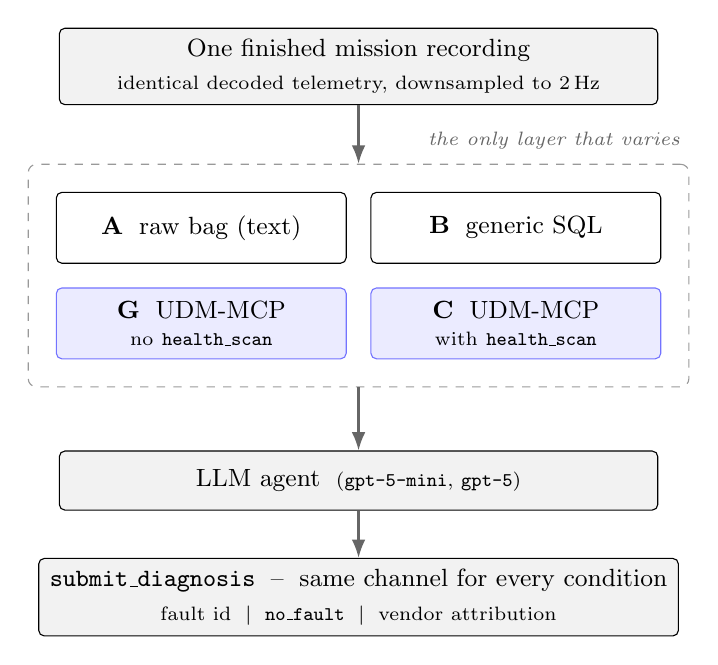
\begin{tikzpicture}[
  font=\small,
  >=Latex,
  box/.style   = {draw, rounded corners=2pt, align=center, inner sep=4pt,
                  minimum height=7.5mm},
  fixed/.style = {box, fill=gray!10, minimum width=76mm},
  iface/.style = {box, text width=34mm, align=center, minimum height=9mm,
                  font=\small},
  base/.style  = {iface, fill=white},
  udm/.style   = {iface, fill=blue!8, draw=blue!55},
  lbl/.style   = {font=\scriptsize\itshape, text=black!60},
]

% --- fixed input -------------------------------------------------------
\node[fixed] (rec) {One finished mission recording\\[1pt]
  \scriptsize identical decoded telemetry, downsampled to 2\,Hz};

% --- the varied layer: four telemetry interfaces -----------------------
\node[base, below left =11mm and 1.5mm of rec.south] (a)
  {\textbf{A}\; raw bag (text)};
\node[base, below right=11mm and 1.5mm of rec.south] (b)
  {\textbf{B}\; generic SQL};
\node[udm, below=3mm of a] (g)
  {\textbf{G}\; UDM-MCP\\[-1pt]\scriptsize no \texttt{health\_scan}};
\node[udm, below=3mm of b] (c)
  {\textbf{C}\; UDM-MCP\\[-1pt]\scriptsize with \texttt{health\_scan}};

\begin{scope}[on background layer]
  \node[draw=black!40, dashed, rounded corners=3pt,
        fit=(a)(b)(g)(c), inner sep=3.5mm] (varied) {};
\end{scope}
\node[lbl, anchor=south east] at ([yshift=0.6mm]varied.north east)
  {the only layer that varies};

% --- agent and fixed answer channel ------------------------------------
\node[fixed, below=8mm of varied.south] (agent)
  {LLM agent \;\scriptsize(\texttt{gpt-5-mini}, \texttt{gpt-5})};
\node[fixed, below=6mm of agent] (ans)
  {\texttt{submit\_diagnosis} \;--\; same channel for every condition\\[1pt]
   \scriptsize fault id \;$|$\; \texttt{no\_fault} \;$|$\; vendor attribution};

% --- wiring ------------------------------------------------------------
\draw[->, thick, black!60] (rec.south) -- (varied.north);
\draw[->, thick, black!60] (varied.south) -- (agent.north);
\draw[->, thick, black!60] (agent.south) -- (ans.north);

\end{tikzpicture}%
}
\caption{The benchmark isolates the data-model layer. Every condition analyses the
\emph{same} recording and commits its answer through the \emph{same} channel; only
the interface between the agent and the telemetry changes. \condG{} removes the
generic triage tool from \condC, separating what the schema does on its own from
what a tool written once against the schema adds.}
\label{fig:design}
\end{figure}


\paragraph{Task} Each run gives an agent exactly one finished mission. The agent
must decide whether a fault occurred and, if so, name it from a fixed 16-fault
catalogue (or answer \texttt{no\_fault}); on multi-vendor missions it must also
attribute the fault to the correct platform. Every condition answers through the
same tool (\texttt{submit\_diagnosis}), so conditions differ only in how the agent
reaches the telemetry, never in how it answers.

\paragraph{Missions and faults} We use 47 missions: 25 single-vendor (TurtleBot3)
and 22 multi-vendor (TurtleBot3 and PX4 in one shared world). Of these, 23 are
faulty and 24 are clean, so a useful agent must both catch real faults and stay
quiet on healthy missions. The catalogue offered to the agent has 16 entries
(9 TurtleBot3, 7 PX4); the faulty missions use 9 of them
(Table~\ref{tab:per-fault}). All conditions see the same recording downsampled to a
common 2\,Hz, so no condition has a temporal-resolution advantage.

\paragraph{Conditions} All conditions share the task and answer channel
(Fig.~\ref{fig:design}):
\begin{itemize}
  \item \condA{} \textbf{Raw bag (text)}: decoded native logs as paginated plain
  text. The ``read the logs'' baseline.
  \item \condB{} \textbf{Generic SQL}: the same telemetry in a SQLite database, one
  table per vendor topic with native column names, queried with \texttt{query\_sql}.
  The ``query the database'' baseline.
  \item \condC{} \textbf{UDM-MCP (full)}: the telemetry normalised into the UDM and
  served over MCP with a structured query surface (\texttt{query\_events},
  \texttt{aggregate}, \texttt{timeline}, \texttt{get\_event} and schema
  introspection), cross-source correlation, a compliance audit, and the triage
  tool \hs{}.
  \item \condG{} \textbf{UDM-MCP $-$ \hs{}}: identical to \condC{} without the
  triage tool.
  \item D and E remove cross-source correlation and the compliance audit
  respectively. We report them at \texttt{gpt-5-mini} only. A third ablation, F
  (schema introspection only), was run with an earlier harness version and is not
  comparable, so we exclude it.
\end{itemize}

\paragraph{The triage tool} \hs{} returns, for every source in the mission, about a
dozen per-source statistics: counts of non-finite IMU and attitude samples, minimum
LiDAR valid fraction and maximum NaN and infinite ray counts, battery minima and
range, angular-rate and speed extremes, and the longest silence on any
continuously published stream. It is implemented entirely as calls to the generic
\texttt{aggregate} tool over UDM field paths, grouped by source, plus a stream-gap
scan over event timestamps. The same code runs on the TurtleBot3 and the PX4
without any per-vendor branch. It contains no fault-specific detector, but its
description to the agent does say which kind of fault each indicator tends to
suggest (for example, non-finite attitude samples suggest IMU saturation). We treat
these hints as part of the tool.

\paragraph{Data plane} Telemetry is ingested into an event store and served
through the shipped UDM-over-MCP server; the agent speaks MCP (JSON-RPC over
stdio). The store used here is \emph{PhyCloud}, an event platform that ingests
heterogeneous sources into \udm{} and exposes them over MCP. Any conformant \udm{}
store would serve the same role, since the agent depends only on the data model and
the protocol. The answer channel is intercepted locally and never forwarded.

\paragraph{Models} We evaluate two model scales from one family,
\texttt{gpt-5-mini} and \texttt{gpt-5}, with fixed decoding settings. A single
model family is a deliberate scope limit (Section~\ref{sec:limitations}).

\paragraph{Metrics} We report a four-way detection breakdown: \emph{found} (faulty
mission, right fault), \emph{missed}, \emph{false alarm} (clean mission, claimed a
fault) and \emph{correct abstain}. From it we derive recall, specificity and
balanced accuracy, each with a percentile bootstrap 95\% CI (10{,}000 resamples,
fixed seed). We also report vendor attribution on multi-vendor faulty missions,
cost per run and tool calls. Scoring is deterministic: a diagnosis is correct only
if the submitted \texttt{fault\_id} matches the ground truth (or is
\texttt{no\_fault} on a clean mission). No model grades another model's answer.

\paragraph{Paired analysis} Every condition runs on the same missions, so we
compare conditions mission by mission. For each pair of conditions and each binary
outcome we run an exact McNemar test~\cite{mcnemar1947} on the discordant missions,
adjust with Holm's procedure~\cite{holm1979} within each (model, outcome) family of
five comparisons, and report Cohen's $h$~\cite{cohen1988} as an effect size. For
recall and balanced-accuracy differences we use a paired bootstrap~\cite{efron1993}
that resamples missions within the faulty and clean strata and applies each draw to
both conditions.

\paragraph{Evidence oracle} To separate ``the agent missed the fault'' from ``the
recording does not contain it'', we compute, for each faulty mission, the one
telemetry statistic that the injected fault's mechanism should move (for example,
the longest gap between GPS samples for a GPS dropout, or the peak gap between
odometry and AMCL pose for odometry drift). A fault counts as \emph{detectable} if
its statistic exceeds the maximum over every clean mission of the same composition
and the faulted robot recorded telemetry at all. The oracle knows which fault to
look for, so it is an upper bound on available evidence, not a fair detector.

% ===========================================================================
\section{Defensibility: Making the Comparison Fair}
% ===========================================================================

% AUTO-GENERATED by paper/gen_tables.py — do not edit by hand.
\begin{table*}[t]
\centering
\caption{Detection breakdown at \texttt{gpt-5} ($n{=}47$: 23 faulty, 24 clean). Conditions ordered by faults \emph{found}. FA = false alarms on clean missions. Bracketed ranges are percentile bootstrap 95\% CIs.}
\label{tab:detection-gpt5}
\small
\resizebox{\textwidth}{!}{%
\begin{tabular}{lccccccr}
\toprule
Condition & Found/Faulty & Recall [95\% CI] & Specificity [95\% CI] & Balanced [95\% CI] & FA & Tools & \$/run \\
\midrule
A: raw bag (text) & 4/23 & 0.17 [0.04, 0.35] & 0.25 [0.08, 0.42] & 0.21 [0.11, 0.34] & 18 & 7.4 & 0.392 \\
B: generic SQL & 2/23 & 0.09 [0.00, 0.22] & 0.88 [0.75, 1.00] & 0.48 [0.40, 0.57] & 3 & 24.3 & 0.163 \\
G: UDM$-$health\_scan & 5/23 & 0.22 [0.04, 0.39] & 0.75 [0.58, 0.92] & 0.48 [0.36, 0.61] & 6 & 18.0 & 0.286 \\
C: UDM$+$health\_scan & 10/23 & 0.43 [0.22, 0.65] & 0.75 [0.58, 0.92] & 0.59 [0.46, 0.72] & 6 & 9.6 & 0.279 \\
\bottomrule
\end{tabular}%
}
\end{table*}

% AUTO-GENERATED by paper/gen_tables.py — do not edit by hand.
\begin{table*}[t]
\centering
\caption{Detection breakdown at \texttt{gpt-5-mini} ($n{=}47$). Same layout as Table~\ref{tab:detection-gpt5}. At this scale $B$'s abstention inflates the balanced scalar while it finds no faults, and no condition exceeds chance (balanced $=0.5$).}
\label{tab:detection-mini}
\small
\resizebox{\textwidth}{!}{%
\begin{tabular}{lccccccr}
\toprule
Condition & Found/Faulty & Recall [95\% CI] & Specificity [95\% CI] & Balanced [95\% CI] & FA & Tools & \$/run \\
\midrule
A: raw bag (text) & 3/23 & 0.13 [0.00, 0.30] & 0.04 [0.00, 0.12] & 0.09 [0.02, 0.17] & 23 & 6.3 & 0.085 \\
B: generic SQL & 0/23 & 0.00 [0.00, 0.00] & 0.83 [0.67, 0.96] & 0.42 [0.33, 0.48] & 4 & 19.4 & 0.057 \\
G: UDM$-$health\_scan & 4/23 & 0.17 [0.04, 0.35] & 0.38 [0.21, 0.58] & 0.27 [0.15, 0.40] & 15 & 17.1 & 0.030 \\
C: UDM$+$health\_scan & 11/23 & 0.48 [0.26, 0.70] & 0.08 [0.00, 0.21] & 0.28 [0.17, 0.39] & 22 & 9.4 & 0.031 \\
\bottomrule
\end{tabular}%
}
\end{table*}


A benchmark that flatters the thing it promotes is marketing, not evidence. Three
issues could bias this comparison.

\paragraph{Pretraining asymmetry (favours the baselines)} The models have seen large
amounts of SQL and ROS and PX4 log data in pretraining and none of the UDM. We give
the UDM conditions a schema orientation in the system prompt to level this gap.
This is a real and permanent cost of any new format, since a deployment must always
describe its schema at inference time, not an advantage handed to the UDM.

\paragraph{Tooling (favours the UDM)} The baselines get no triage tool, and this is
deliberate. An equivalent tool for \condA{} or \condB{} would have to be written
against each vendor's native topics, message types and column names, and rewritten
for every vendor added, which is precisely the per-vendor integration cost a shared
data model is meant to remove. \hs{} exists in the UDM condition because the schema
makes it a few generic queries. We therefore report two contrasts and keep them
separate: \condC{} against the baselines measures the UDM surface as it would be
deployed, tooling included; \condG{} against the baselines measures the schema
without that tool. We also hold to a fairness contract: no answer leakage, no
fault-specific detectors, and no data that the baselines lack, since every
condition is derived from the same recording.

\paragraph{Unanswerable faults (affects all conditions)} If a fault leaves no trace,
no condition can find it, and counting it lowers every recall equally. We measure
this directly with the evidence oracle (Section~\ref{sec:evidence}) and report
results both on all faults and on the faults that leave evidence.

% ===========================================================================
\section{Results}
% ===========================================================================

\subsection{Detection}
At \texttt{gpt-5} (Table~\ref{tab:detection-gpt5}), the full UDM surface (\condC)
finds 10 of 23 faults, against 5 for the tool-free ablation (\condG), 4 for raw logs
(\condA) and 2 for SQL (\condB). At \texttt{gpt-5-mini}
(Table~\ref{tab:detection-mini}) the ordering is the same: 11, 4, 3 and 0.

% AUTO-GENERATED by paper/gen_tables.py — do not edit by hand.
\begin{table*}[t]
\centering
\caption{Paired comparisons on the same missions. Each McNemar cell is the discordant split $b$--$c$ ($b$: only the first condition correct; $c$: only the second) with the exact $p$, Holm-adjusted over the five comparisons in its (model, metric) family. Found: $23$ faulty missions; Abstain: $24$ clean; Vendor: $13$ multi-vendor faulty. $\Delta$Recall is the paired-bootstrap difference with 95\% CI; bold marks Holm $p<0.05$ or a CI excluding $0$.}
\label{tab:paired}
\small
\resizebox{\textwidth}{!}{%
\begin{tabular}{lcccccccc}
\toprule
 & \multicolumn{4}{c}{gpt-5} & \multicolumn{4}{c}{gpt-5-mini} \\
\cmidrule(lr){2-5} \cmidrule(lr){6-9}
Pair & Found & Abstain & Vendor & $\Delta$Recall [95\% CI] & Found & Abstain & Vendor & $\Delta$Recall [95\% CI] \\
\midrule
C vs A & 7--1 (.250) & \textbf{16--4 (.047)} & 6--3 (1.000) & \textbf{+0.26 [+0.04, +0.48]} & 9--1 (.064) & 2--1 (1.000) & 5--1 (.438) & \textbf{+0.35 [+0.13, +0.57]} \\
C vs B & \textbf{8--0 (.039)} & 3--6 (1.000) & 9--1 (.107) & \textbf{+0.35 [+0.17, +0.57]} & \textbf{11--0 (.005)} & \textbf{1--19 ($<$.001)} & \textbf{11--0 (.005)} & \textbf{+0.48 [+0.26, +0.70]} \\
C vs G & 5--0 (.250) & 4--4 (1.000) & 1--1 (1.000) & \textbf{+0.22 [+0.09, +0.39]} & 7--0 (.062) & \textbf{0--7 (.031)} & 5--0 (.188) & \textbf{+0.30 [+0.13, +0.48]} \\
G vs A & 2--1 (1.000) & \textbf{13--1 (.009)} & 6--3 (1.000) & +0.04 [$-$0.09, +0.17] & 3--2 (1.000) & \textbf{8--0 (.030)} & 2--3 (1.000) & +0.04 [$-$0.13, +0.22] \\
G vs B & 5--2 (.906) & 2--5 (1.000) & 9--1 (.107) & +0.13 [$-$0.09, +0.35] & 4--0 (.250) & \textbf{2--13 (.030)} & 6--0 (.125) & \textbf{+0.17 [+0.04, +0.35]} \\
\bottomrule
\end{tabular}%
}
\end{table*}


The paired comparisons (Table~\ref{tab:paired}) show which of these gaps the sample
resolves. \condC{} finds more faults than \condB{} at both scales, with no mission
going the other way (8--0, Holm $p=0.039$; 11--0, Holm $p=0.005$). Against raw logs
the discordant splits are 7--1 and 9--1. Those miss the Holm threshold ($p=0.25$ and
$p=0.064$), but the paired recall differences, $+0.26$ $[+0.04, +0.48]$ and $+0.35$
$[+0.13, +0.57]$, exclude zero at both scales. The full UDM surface is the
strongest detector at both scales.

\subsection{An evidence ceiling: 7 of 23 faults leave no trace}
\label{sec:evidence}
% AUTO-GENERATED by paper/gen_tables.py — do not edit by hand.
\begin{table*}[t]
\centering
\caption{Faults found by fault type. \emph{Evid.}\ counts the missions on which a fault-aware oracle sees the fault's signal in the recording (above every clean mission of the same composition). No condition at either scale found a fault the oracle could not see.}
\label{tab:per-fault}
\small
\begin{tabular}{lcccccccccc}
\toprule
 & & & \multicolumn{4}{c}{gpt-5} & \multicolumn{4}{c}{gpt-5-mini} \\
\cmidrule(lr){4-7} \cmidrule(lr){8-11}
Fault & $n$ & Evid. & A & B & G & C & A & B & G & C \\
\midrule
\texttt{px4\_gps\_dropout} & 5 & 5 & 0 & 1 & 0 & 3 & 0 & 0 & 0 & 3 \\
\texttt{px4\_imu\_saturation} & 4 & 4 & 2 & 0 & 4 & 4 & 1 & 0 & 2 & 4 \\
\texttt{tb3\_costmap\_inflation\_drift} & 1 & 1 & 0 & 0 & 0 & 0 & 1 & 0 & 0 & 0 \\
\texttt{tb3\_imu\_bias} & 2 & 2 & 1 & 0 & 0 & 0 & 0 & 0 & 0 & 0 \\
\texttt{tb3\_lidar\_dropout} & 1 & 1 & 0 & 1 & 0 & 1 & 1 & 0 & 0 & 1 \\
\texttt{tb3\_lidar\_noise} & 3 & 3 & 1 & 0 & 1 & 2 & 0 & 0 & 2 & 3 \\
\texttt{tb3\_map\_mismatch} & 1 & 0 & 0 & 0 & 0 & 0 & 0 & 0 & 0 & 0 \\
\texttt{tb3\_motor\_stall} & 3 & 0 & 0 & 0 & 0 & 0 & 0 & 0 & 0 & 0 \\
\texttt{tb3\_odometry\_drift} & 3 & 0 & 0 & 0 & 0 & 0 & 0 & 0 & 0 & 0 \\
\midrule
All & 23 & 16 & 4 & 2 & 5 & 10 & 3 & 0 & 4 & 11 \\
\bottomrule
\end{tabular}
\end{table*}


The oracle finds a visible signal for 16 of the 23 faulty missions
(Table~\ref{tab:per-fault}). The seven without one are all three odometry drifts,
all three motor stalls and the map mismatch. Their discriminating signals, such as
the true pose, wheel commands before they reach the drive, and the world model, are
not in the recording, and one of the motor stalls is on a multi-vendor mission where
the TurtleBot3 recorded no telemetry at all. Independently of the oracle, no
condition at either scale found any of these seven faults (0 of 56 runs). Every
recall figure in this paper therefore has a ceiling of $16/23 \approx 0.70$.

The ceiling falls unevenly across compositions. All nine PX4 faults leave strong
evidence (GPS gaps 13 times longer than on any clean mission; hundreds of
non-finite attitude samples), and so do 12 of the 13 multi-vendor faults. Only 4 of
the 10 single-vendor faults do. This matters for the composition comparison below.

% AUTO-GENERATED by paper/gen_tables.py — do not edit by hand.
\begin{table}[t]
\centering
\caption{Detection on the 16 faulty missions whose fault leaves evidence, with all 24 clean missions. Balanced accuracy with bootstrap 95\% CI.}
\label{tab:evidence-restricted}
\footnotesize
\resizebox{\columnwidth}{!}{%
\begin{tabular}{lcccc}
\toprule
 & \multicolumn{2}{c}{gpt-5} & \multicolumn{2}{c}{gpt-5-mini} \\
\cmidrule(lr){2-3} \cmidrule(lr){4-5}
Condition & Found & Balanced & Found & Balanced \\
\midrule
A: raw bag (text) & 4/16 & 0.25 [0.11, 0.40] & 3/16 & 0.11 [0.02, 0.23] \\
B: generic SQL & 2/16 & 0.50 [0.40, 0.60] & 0/16 & 0.42 [0.33, 0.48] \\
G: UDM$-$health\_scan & 5/16 & 0.53 [0.39, 0.68] & 4/16 & 0.31 [0.18, 0.46] \\
C: UDM$+$health\_scan & 10/16 & 0.69 [0.54, 0.82] & 11/16 & 0.39 [0.25, 0.51] \\
\bottomrule
\end{tabular}%
}
\end{table}


Restricted to the 16 evidence-bearing faults (Table~\ref{tab:evidence-restricted}),
\condC{} finds 10 at \texttt{gpt-5} and 11 at \texttt{gpt-5-mini}, and its
balanced accuracy at \texttt{gpt-5} is $0.69$ $[0.54, 0.82]$, the only interval in
the study that lies entirely above chance.

\subsection{Where the detection gain comes from}
Removing \hs{} costs detection at both scales: on every mission where \condC{} and
\condG{} disagree about a faulty mission, \condC{} is right (5--0 at \texttt{gpt-5},
7--0 at \texttt{gpt-5-mini}, 12--0 pooled), and the paired recall differences,
$+0.22$ and $+0.30$, exclude zero. Without the tool, the UDM surface finds about as
many faults as raw logs (5 vs.\ 4 and 4 vs.\ 3; recall differences $+0.04$ at both
scales). The schema alone does not make the agent a better detector.

The other ablations change nothing measurable. At \texttt{gpt-5-mini}, removing
cross-source correlation (D) leaves detection at 11/23 (2--2 discordant), and
removing the compliance audit (E) gives 9/23 (4--2). Among the UDM tools, only
\hs{} matters for detection.

We read this as evidence for the mechanism behind the data model's value rather
than against it. \hs{} is a short composition of generic aggregate queries that
runs unchanged on both vendors' data. Writing its equivalent against the raw
formats would mean one implementation per vendor. The schema is what makes a
general-purpose diagnostic tool cheap to write and portable across a fleet, and
that tool is what finds the faults. What this benchmark does not show is that
presenting the data in a uniform schema, with no tooling on top, improves
detection by itself.

\subsection{Calibration: what the schema does on its own}
The tool-free comparison does show one structural effect. At \texttt{gpt-5}, raw
logs raise 18 false alarms on 24 clean missions; both UDM conditions raise 6. Paired,
\condG{} abstains correctly where \condA{} does not on 13 clean missions and the
reverse on 1 (Holm $p=0.009$), and \condC{} splits 16--4 against \condA{} (Holm
$p=0.047$). At \texttt{gpt-5-mini} \condG{} still beats raw logs on clean missions
(8--0, Holm $p=0.030$). The structured surface makes the agent stop guessing on
healthy telemetry, with or without the triage tool. Raw logs' false alarms have a
recognisable source: at \texttt{gpt-5}, 9 of them claim a LiDAR dropout, because a
healthy scan routinely contains 25--33\% out-of-range rays, which read as missing
data in plain text.

This benefit has a limit at the smaller scale. At \texttt{gpt-5-mini}, \hs{} makes
the agent over-alarm: \condC{} abstains correctly on only 2 of 24 clean missions
against 9 for \condG{} (0--7, Holm $p=0.031$), and 11 of its 22 false alarms claim
LiDAR noise, which suggests the smaller model over-reads the tool's LiDAR summary.
\condC{}'s higher recall at that scale therefore partly reflects a readier
willingness to name a fault rather than better discrimination; its balanced
accuracy ($0.28$) is below chance.

\subsection{The balanced scalar is gamed by abstention}
SQL posts competitive balanced accuracy ($0.48$ at \texttt{gpt-5}, $0.42$ at
\texttt{gpt-5-mini}) while finding 2 and 0 faults. It scores by declining to answer:
it has the most correct abstentions at both scales (21 and 20 of 24). A single
balanced number would rank it alongside the UDM conditions; the breakdown shows
that it does not diagnose. Fig.~\ref{fig:detection-scatter} plots faults found
against false alarms. The chance frontier is the diagonal $\text{found}/23 =
\text{FA}/24$, and only \condC{} at \texttt{gpt-5} lies above it.

% AUTO-GENERATED by paper/gen_tables.py — do not edit by hand.
\begin{table}[t]
\centering
\caption{Cross-vendor attribution on multi-vendor faulty missions ($n{=}13$ per cell): did the agent blame the correct platform (TurtleBot3 vs.\ PX4)? Reported at both model scales.}
\label{tab:cross-vendor}
\footnotesize
\resizebox{\columnwidth}{!}{%
\begin{tabular}{lcccc}
\toprule
 & \multicolumn{2}{c}{gpt-5} & \multicolumn{2}{c}{gpt-5-mini} \\
\cmidrule(lr){2-3} \cmidrule(lr){4-5}
Condition & Vendor & Found & Vendor & Found \\
\midrule
A: raw bag (text) & 7/13 & 3/13 & 7/13 & 1/13 \\
B: generic SQL & 2/13 & 1/13 & 0/13 & 0/13 \\
G: UDM$-$health\_scan & 10/13 & 4/13 & 6/13 & 4/13 \\
C: UDM$+$health\_scan & 10/13 & 8/13 & 11/13 & 9/13 \\
\bottomrule
\end{tabular}%
}
\end{table}

% AUTO-GENERATED by paper/gen_tables.py — do not edit by hand.
\begin{figure}[t]
\centering
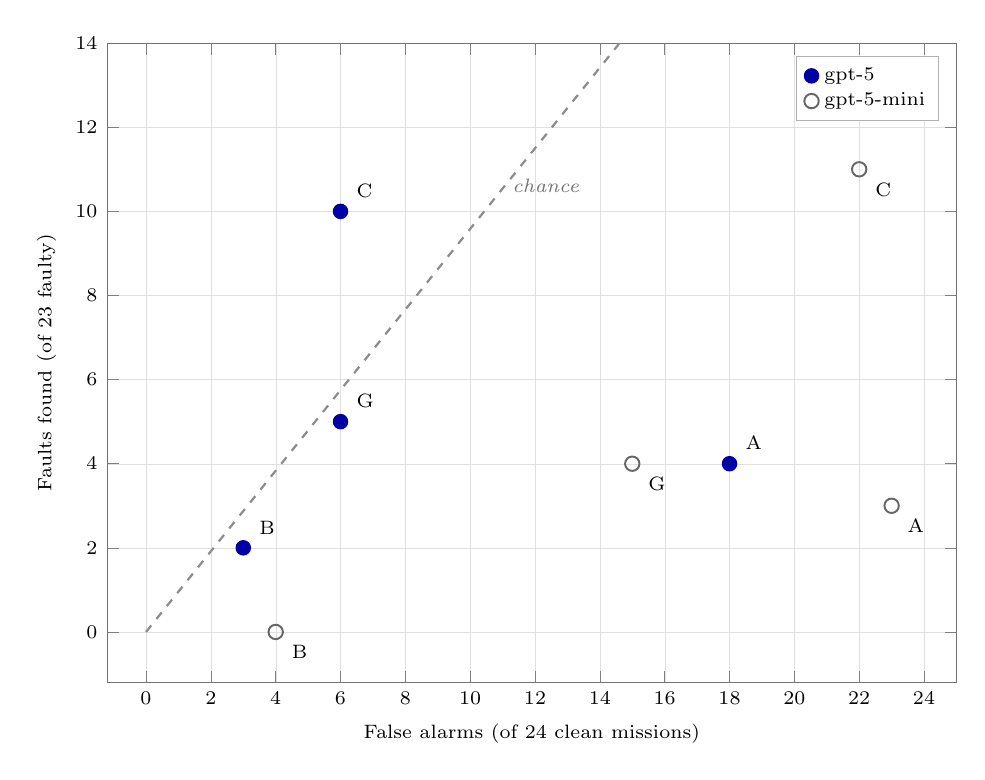
\begin{tikzpicture}
\begin{axis}[
  width=1.02\columnwidth, height=0.80\columnwidth,
  xlabel={False alarms (of 24 clean missions)},
  ylabel={Faults found (of 23 faulty)},
  xmin=-1.2, xmax=25, ymin=-1.2, ymax=14,
  grid=both,
  major grid style={line width=0.1pt, draw=black!12},
  tick label style={font=\scriptsize},
  label style={font=\scriptsize},
  legend style={font=\scriptsize, at={(0.98,0.98)}, anchor=north east,
                draw=black!30, fill=white, row sep=-1pt},
  legend cell align=left,
  axis line style={black!55},
]
\addplot[domain=0:24, samples=2, dashed, black!45, thick,
         forget plot] {23/24*x};
\node[font=\scriptsize\itshape, text=black!55, anchor=north west]
  at (axis cs:11,11) {chance};
\addplot[only marks, mark=*, mark size=2.6pt, draw=blue!65!black,
         fill=blue!65!black] coordinates {(18,4) (3,2) (6,5) (6,10)};
\addlegendentry{gpt-5}
\addplot[only marks, mark=o, mark size=2.6pt, draw=black!60,
         line width=0.7pt] coordinates {(23,3) (4,0) (15,4) (22,11)};
\addlegendentry{gpt-5-mini}
\node[above right=0.5mm and 0.8mm, font=\scriptsize] at (axis cs:18,4) {A};
\node[above right=0.5mm and 0.8mm, font=\scriptsize] at (axis cs:3,2) {B};
\node[above right=0.5mm and 0.8mm, font=\scriptsize] at (axis cs:6,5) {G};
\node[above right=0.5mm and 0.8mm, font=\scriptsize] at (axis cs:6,10) {C};
\node[below right=0.5mm and 0.8mm, font=\scriptsize] at (axis cs:23,3) {A};
\node[below right=0.5mm and 0.8mm, font=\scriptsize] at (axis cs:4,0) {B};
\node[below right=0.5mm and 0.8mm, font=\scriptsize] at (axis cs:15,4) {G};
\node[below right=0.5mm and 0.8mm, font=\scriptsize] at (axis cs:22,11) {C};
\end{axis}
\end{tikzpicture}
\caption{Faults found vs.\ false alarms, both model scales. The dashed line is the chance frontier (balanced accuracy $=0.5$): a condition beats a coin flip only above it. Exactly one point clears it---the full UDM surface at \texttt{gpt-5}. \condB{} hugs the origin by abstaining; \condA{} and \condC{} at \texttt{gpt-5-mini} sit far right by over-alarming.}
\label{fig:detection-scatter}
\end{figure}


\subsection{Cross-vendor attribution}
The reason to adopt a vendor-neutral model is mixed fleets, so the sharpest test is
whether the agent blames the right platform when a TurtleBot3 and a PX4 run
together. \condC{} attributes correctly on 10 of 13 multi-vendor faulty missions at
\texttt{gpt-5} and 11 of 13 at \texttt{gpt-5-mini}
(Table~\ref{tab:cross-vendor}), against 7 for raw logs at both scales and 2 and 0
for SQL. Against SQL the gap is large at both scales (9--1 and 11--0 discordant;
Holm $p=0.107$ and $p=0.005$). Against raw logs it is in the same direction but not
resolved by 13 missions. The two baselines fail in different ways. Raw logs mostly
blame the wrong robot: 6 of \condA{}'s 9 misses on evidence-bearing multi-vendor
faults at \texttt{gpt-5} name the wrong vendor. SQL mostly never answers: at
\texttt{gpt-5-mini}, 10 of its 12 such misses end without a diagnosis, the agent
having spent its budget exploring per-vendor tables. Without \hs{}, attribution
holds at \texttt{gpt-5} (10/13) but drops to the raw-log level at
\texttt{gpt-5-mini} (6/13).

\subsection{Single- vs.\ multi-vendor missions}
The hypothesis that motivated the benchmark is that a UDM loses less accuracy than
the baselines as a fleet becomes heterogeneous. This mission set cannot test it.
\condC{}'s recall is in fact higher on multi-vendor missions ($+0.42$ at
\texttt{gpt-5}, $+0.49$ at \texttt{gpt-5-mini}, both CIs excluding zero), but the
two mission sets do not share a fault mix: multi-vendor missions carry all nine PX4
faults, which leave strong evidence, while single-vendor missions carry six of the
seven faults that leave none. Restricted to TurtleBot3 faults only, or to
evidence-bearing faults only, no condition's composition difference, and no
difference between conditions in that difference, excludes zero. Vendor attribution
above is the cross-vendor result the data supports.

\subsection{Cost}
At \texttt{gpt-5}, the UDM conditions cost about \$0.28 per run against \$0.39 for
raw logs (Table~\ref{tab:detection-gpt5}); the raw-log context, hundreds of
thousands of tokens of decoded text per mission, dominates. SQL is cheapest per run
(\$0.16) but finds almost nothing. Per fault found over the 47 missions, \condC{}
costs \$1.31, against \$2.69 for \condG, \$3.84 for \condB{} and \$4.60 for
\condA. \condC{} also uses the fewest tool calls of any condition that finds faults
(9.6 per run, against 18.0 for \condG{} and 24.3 for \condB).

% ===========================================================================
\section{Discussion: Implications for an Open Ecosystem}
% ===========================================================================

The results separate two things a unified data model could offer. The first is
\emph{presentation}: whether the agent reasons better when every vendor's data has
the same shape. On detection, the answer here is no; the tool-free UDM surface finds
about as many faults as raw logs. It does reduce false alarms at both scales and
keeps vendor attribution high at the larger scale. The second is \emph{tooling}:
whether a shared schema lets diagnostic tools be written once and used everywhere.
Here the effect is large. A dozen generic aggregate queries, written once against
the schema with no per-vendor code, account for the detection gain at both scales,
and the full surface beats both baselines on detection and SQL on attribution.

For a mixed fleet, the second effect is the one that matters operationally. The
baselines could in principle be given an equivalent tool, but only by writing it
once per vendor and again whenever a vendor changes its format. The data model turns
that $O(\text{tools} \times \text{vendors})$ cost into $O(\text{tools} +
\text{vendors})$, and our results show that, for LLM fault diagnosis, the tools are
where the accuracy comes from. An open standard extends this: anyone can write a
tool against it, and the tool works on every conformant source. Realising this in
production requires the events to exist somewhere queryable at operational scale,
a serving layer that ingests heterogeneous sources into the model and exposes them
through a standard interface such as MCP.

% ===========================================================================
\section{Limitations}
\label{sec:limitations}
% ===========================================================================

\begin{itemize}
  \item \textbf{No tool-matched baseline.} We did not build per-vendor triage tools
  for the baselines, for the reason given above. The comparison of \condC{} with
  the baselines therefore measures a data model together with the tooling it
  enables, not the schema in isolation; \condG{} isolates the schema.
  \item \textbf{Single model family.} We evaluate only the \texttt{gpt-5} family.
  Generality across model families is the most important open question.
  \item \textbf{One run per mission.} Each mission is run once per condition, so
  decoding variance is not separated from mission-to-mission variance.
  \item \textbf{Sample size.} With 23 faulty, 24 clean and 13 multi-vendor faulty
  missions, several directional results, including \condC{} vs.\ \condA{} on
  detection after Holm correction and on attribution, are not resolved.
  \item \textbf{Confounded composition.} The single- and multi-vendor mission sets
  differ in fault mix and in evidence (4/10 vs.\ 12/13 detectable), so the
  heterogeneity hypothesis is untested. A matched design, in which every fault type
  with a recordable signal appears equally often on both compositions, would test
  it.
  \item \textbf{Evidence ceiling and data quality.} Seven faults leave no trace;
  three multi-vendor missions recorded no TurtleBot3 telemetry. The oracle is
  fault-aware and has thin margins on some faults (IMU bias clears the clean
  maximum by about 1.3 times), so ``detectable'' is an upper bound.
  \item \textbf{Tool hints.} \hs{}'s description maps indicators to fault kinds.
  This is generic domain knowledge rather than a fault detector, but it is
  knowledge the baselines are not given.
  \item \textbf{Simulated, scripted faults.} All missions come from one simulator,
  and faults are injected by script with known onset, so they may be cleaner than
  faults in the field. A second simulator, real-robot data and independent UDM
  implementations would strengthen external validity.
  \item \textbf{Offline, English-only.} Agents analyse a finished mission in batch
  rather than a live stream, and all prompts are in English.
\end{itemize}

% ===========================================================================
\section{Conclusion}
% ===========================================================================

Holding task, data and answer format fixed and varying only the telemetry
interface, an open vendor-neutral data model served over MCP made LLM fault
diagnosis better at finding faults than raw logs and SQL, and better at
attributing faults across vendors than SQL, at two model scales and at lower cost
per fault found. At the larger scale, on faults that leave evidence, it was the only
condition clearly above chance. The ablation shows how: the schema by itself makes
the agent better calibrated, and a generic triage tool, written once against the
schema and run unchanged on every vendor, supplies the detection gain. Nearly a third of
the injected faults left no trace for any condition to find, and the mission set
cannot test whether the benefit grows with heterogeneity. Extending the evaluation
to other model families, repeated runs and a composition-matched fault design are
the natural next steps. The baselines, the scoring and analysis code, the scored
results and the data model are released so others can take them.

% ===========================================================================
\section*{Reproducibility and Availability}
% ===========================================================================
\paragraph{Released} Under Apache-2.0 at
\url{https://github.com/Phyware-Labs/udm-bench}: the scored record of every run
reported here; the scoring suite, including the hallucination detector and the
hand-labelled corpus that validates it; the paired and evidence analyses with a
snapshot of per-run outcomes and per-mission telemetry statistics; the harness
with conditions \condA{} and \condB{} and their prompts; the scenario manifests and
fault taxonomy; and the simulation environment. The \udm{} specification, schemas
and MCP server are released separately~\cite{phyudm}. Every table in this paper is
generated from the scored records by \texttt{paper/gen\_tables.py}, so every
reported number, interval and test can be recomputed; no number in a table is
transcribed by hand.

\paragraph{Not released} The implementations of the UDM conditions
(\condC--\condG) and their prompts, the fault injectors and mission runner, the
ingest pipeline that normalised recordings into \udm{}, and the raw tool-call
traces and mission recordings. None is needed to verify the reported results;
they are needed to re-run conditions \condC--\condG{} or to record new faulted
missions.

\paragraph{Competing interests} The author founded PhyWare Labs, which develops
\udm{} and the PhyCloud event platform used as the data plane in this study. The
study received no external funding; model usage was paid for with cloud credits.

\balance
\bibliographystyle{IEEEtran}
\bibliography{references}

\end{document}
